%!TEX root=thesis.tex
%This is the draft literature review. 

%!TEX ROOT = thesis.tex


\chapter{Background Studies}
\label{section:litreview}

In this chapter, related theoretical background concepts are first introduced. Then, the related state of the art works are discussed in two main portions: 
\begin{enumerate}
    \item Existing methodology and techniques used for semantics extraction
    \item Recent methodology and techniques used for semantic retrieval.
\end{enumerate}



\section{Related Theoretical Background Concepts}
\label{subsec:relatedConcepts}

Before diving deeper into the nitty-gritty of the proposed framework, fundamental understanding towards related theoretical background concepts used in this work is discussed. As this work covers a rather broad spectrum of different concepts, a general understanding towards these concepts would provide some degree of clarity towards the topic at hand. This section briefly describes the fundamental of the following concepts: i) Quantization, ii) Distance Measure, iii) Human Visual System, \& iv) Color Model and Color Terms. 


\subsection{Quantization}

The use of quantization in the mathematical and digital signal processing field is not a new concept. Digital signal processors are limited by natural boundaries such as hardware limitations, and are only able to compute and perform arithmetic operations within a limited range \cite{spors_2018}. The use of quantization refers to the process of mapping and projecting a set of large values which are often continuous or analog in nature into a set of discrete and finite values. 

\begin{figure}[hbt!]\centering
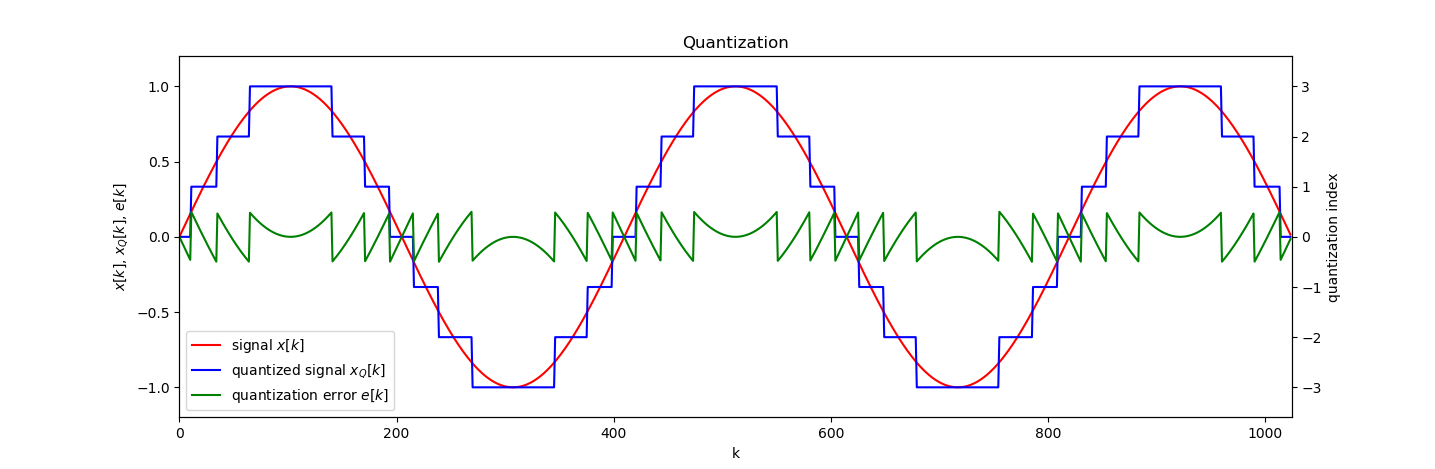
\includegraphics[width=\textwidth]{image/general/quantization.png}
\caption{Quantization}
\label{fig:quantize}
\end{figure}


The use of quantization enables reduction in memory usage (compression) as well as the reduction of computational cost, hence, leading to faster processing speed. However, since the quantization process is a many-to-few mapping operation, the operation is considered irreversible without prior knowledge of the loss. Nevertheless, the output discrete signal can closely resemble the continuous input signal depending on the number of quantization level used.
\begin{equation}\centering
\label{eq:quantization}
x_Q[k] = g( \mspace{3mu}\lfloor \mspace{3mu}f(x[k]) \mspace{3mu}\rfloor\mspace{3mu})
\end{equation} 
\vspace{-3em}
\begin{equation}\centering
\label{eq:quantizationerror}
e[k] = x_Q[k] - x[k]
\end{equation}
In order to expound on the quantization process, a mathematical model of this process can be formulated as such. Consider a continuous signal $x[k]$ whose quantized signal, $x_Q[k]$, is desired (see Equation \ref{eq:quantization}). The functions $f (\mspace{3mu} \cdot  \mspace{3mu})$ \& $g (\mspace{3mu} \cdot  \mspace{3mu})$ can be thought of as a real-value mapping function while the $\lfloor \mspace{3mu} \cdot  \mspace{3mu} \rfloor$ represents a rounding function. The $f (\mspace{3mu} \cdot  \mspace{3mu})$ function is used to convert real-world values into a digital signal, while $g (\mspace{3mu} \cdot  \mspace{3mu})$ is used to map the digital signal into a quantized signal. As previously mention, this process is considered irreversible with prior knowledge of the loss, in this case, the quantization error, $e[k]$, can be computed as Equation \ref{eq:quantizationerror}. Figure \ref{fig:quantize} illustrates a quantization process where the red signal ($x[k]$) represents the real-world continuous signal, the blue signal ($x_Q[k]$) refers to the quantized signal while the green signal ($e[k]$) represents the error due to quantization process.

In order to leverage on this concept, in this work, the quantization technique was extended further into a three dimensional space. As video data can be represented in a 3D space, the quantization process was used to quantize the continuous video data into a set of discrete and finite values. These discrete and finite values can ease the calculation and manipulation of data. As color space can also be represented using a 3D space, this concept was adapted and applied here to quantize the color space into color terms (See Section \ref{section:colorterm}).



\subsection{Distance Measure}
\label{section:distancemeasures}

The use of distance measure is another recurring key concept in the proposed method. Given that distance measures are commonly used in computer science as well as the mathematics field, there are numerous metrics suggested by different authors which are applicable and useful in different scenarios. In essence, distance measure is used to compute the difference between targets. On the flip side, the difference can also be thought of as the similarity between these targets.

\begin{figure}[hbt!]\centering
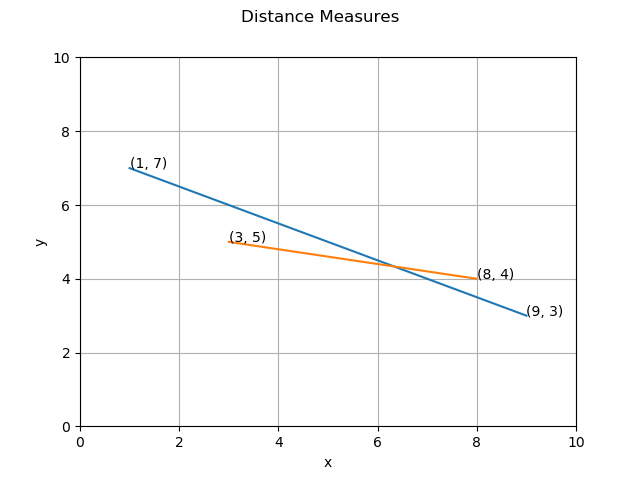
\includegraphics[width=.7\textwidth]{image/general/distance.png}
\caption{Example of Distance Measure}
\label{fig:distanceMeasure}
\end{figure}

To further accentuate on the concept of distance measure in this work, a simple example of how distance metrics can be applied in the proposed method is illustrated using Figure \ref{fig:distanceMeasure} with two plotted lines. In order to simplify the research problem, these lines can be thought of as vehicle trajectories captured over time that is flatten unto a 2D plot. Using the available data, the distance between two trajectories can be measured and used to signify the dissimilarity between them. This distance measure can also be used to identify trajectories with high resemblance. 

However, as different distance measure metrics are suitable for different scenarios, a good distance measure is an essential for comparing a significantly extensive set of vehicle trajectories during the retrieval process of a car park scene. This concept of distance measure was further extended into a multi-dimensional space such as the colors space, where the similarity between two or more colors were measured using different distance metrics to evaluate the performance of each metric. Table \ref{table:distance} lists out several distance measure which are commonly used along with the pros and cons of each while Figure \ref{fig:manhattan} shows the contrast between Euclidean and Manhattan distance.

\begin{table}[]
\label{table:distance}
\resizebox{\textwidth}{!}{
\begin{tabular}{|l|l|l|}
\hline
\textbf{Distance Measure} & \textbf{Pros} & \textbf{Cons}  \\ \hline
Euclidean Distance        & 
\begin{tabular}[c]{@{}l@{}}Simple, \\ Fast, \\ Commonly used\end{tabular}   &
\begin{tabular}[c]{@{}l@{}}Vector order dependent,\\ Requires same length vectors\end{tabular} \\ \hline
Manhattan Distance        & 
\begin{tabular}[c]{@{}l@{}}Reflection invariant, \\ Translation invariant,\\ Produces same distance\end{tabular}  & 
\begin{tabular}[c]{@{}l@{}}Requires same length vectors,\\ Does not have a unique solution\end{tabular} \\ \hline
Chamfer Distance          & 
\begin{tabular}[c]{@{}l@{}}Able to work with \\different length vectors,\\ Vector order invariant, \\ Minimizes the difference \\between vectors\end{tabular} & 
Higher computational cost \\ \hline
\end{tabular}}
\end{table}



\begin{figure}[hbt!]\centering
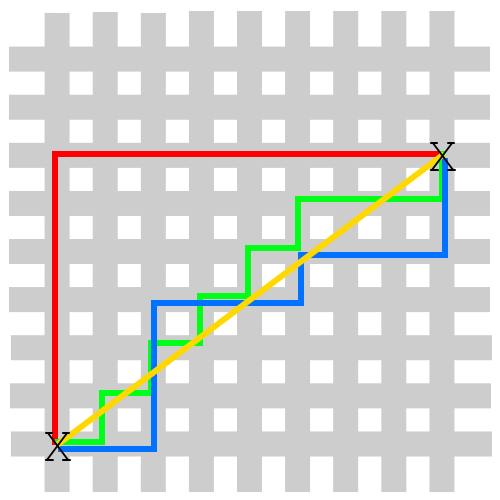
\includegraphics[width=.5\textwidth]{image/lit/manhattan.png}
\caption{Using Manhattan Distance, regardless of the path taken, the distance for the red, green and blue lines has the length of $14$. However, using Euclidean Distance, the distance is measured to be $\sqrt{8^2+6^2} = 10$. Euclidean Distance only produces $1$ unique solution while Manhattan Distance may produce more than one solution.}
\label{fig:manhattan}
\end{figure}


\subsection{Human Visual System}
\label{section:eyes}
The human eyes are visual system organs, responsible of receiving and processing visual information. Figure \ref{fig:eyes} shows a rough anatomy of the human eye. Within the eye, rods and cones are light-sensitive cells, found on the retina which are in charge of vision. While rods cells are not able to perceive colour information, they are known to be responsible for low-light achromatic vision. On the other hand, cones cells are responsible for the reception of color information.   


\begin{figure}[hbt!]\centering
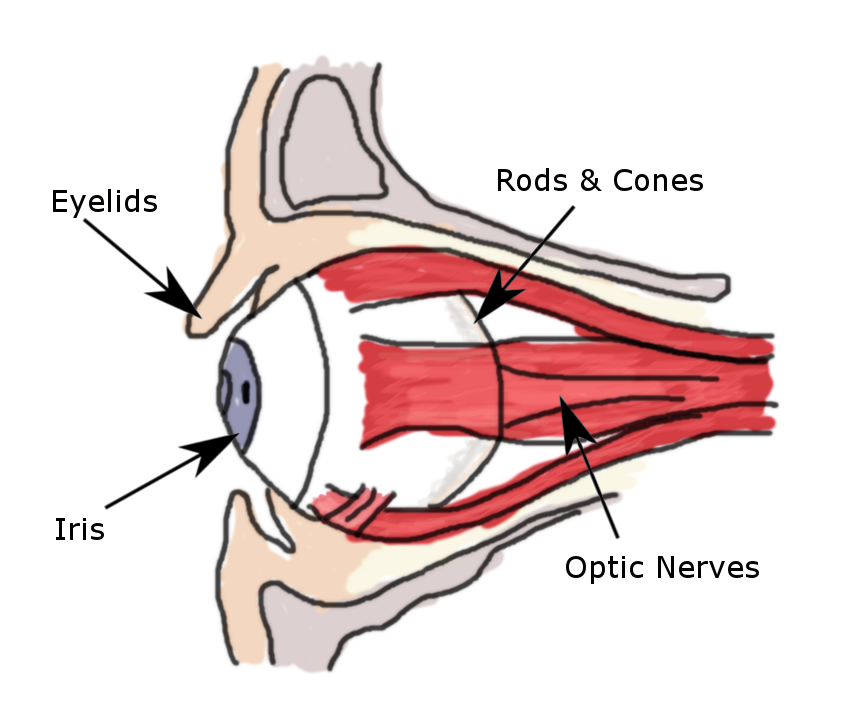
\includegraphics[width=.5\textwidth]{image/lit/rodsandconscolored.png}
\caption{Human Eye Anatomy}
\label{fig:eyes}
\end{figure}

Anatomically, there are three types of cones in the human retina, each of which are responsible over the receptiveness of colors in a particular type of wavelength. These wavelengths can be classified into three main categories: Short wavelengths light ('blue' cones, 420–440 nm), Medium  wavelengths light ('green' cones, 534–545 nm) and Long wavelengths light ('red' cones, 564–580 nm). Colors are perceived from the combination of stimuli to these rods and cones cells and responses from brain. When stimulated, these cells fires electrical signals to the optic nerves fibres that communicates with the brain. However, as the number of cones cells in the retina varies for each person, the color perception of everyone would differ in a way or another. 






\subsection{Color Model and Color Terms}
\label{section:colorterm}

%[cref010219-continue from here]
The humans' visible spectrum $(400nm - 700nm)$ can be represented using the respective wavelengths. In order to describe these values 

\cc{create a table: rgb: how many colors, x11 how many color, munsell: x number of color etc}
https://people.csail.mit.edu/jaffer/Color/Dictionaries
%https://en.wikipedia.org/wiki/Cone_cell

\cc{to fill up... talk about color space and why}
%http://markkness.net/colorpy/ColorPy.html

\begin{figure}[hbt!]\centering
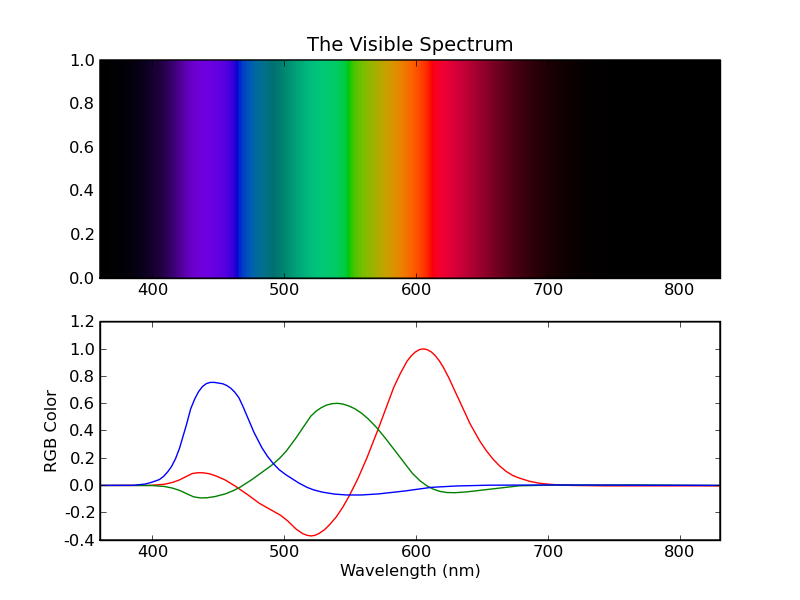
\includegraphics[width=.7\textwidth]{image/general/VisibleSpectrum.png}
\caption{RGB Values and their corresponding spectrum}
\label{fig:visibleSpectrum}
\end{figure}


\subsection{Munsell Color System}
\label{section:munsellcs}
Color terms - such as "Red", "Green" or "Blue", are commonly derived from the Munsell Color system which was created in the early 20th century by Professor Albert H. Munsell. The Munsell Color System was designed to organize colors similar to how the human's eye sees - which is, by organizing colors according to their hues, followed by the chromatic range and the brightness values in a perceptually uniform manner. 

For each horizontal circle on the Munsell Color System, the hues can be divided into 5 principle hues which are Red, Yellow, Green, Blue, and Purple. This setup allows another 5 intermediate hues in between each principle hues, for example: Green-Blue hue, Purple-Red hue. 
Figure \ref{fig:munsell}(a) illustrates the Munsell Color System while Figure \ref{fig:munsell}(b) illustrates the property of the chroma and value scale available on the Munsell color system, for example, a hue at 2.5 Yellow-Red (YR) has a maximum chroma value which differs along the value axis. 



\begin{figure}[!htb]
  \centering
\begin{tabular}{cc}
 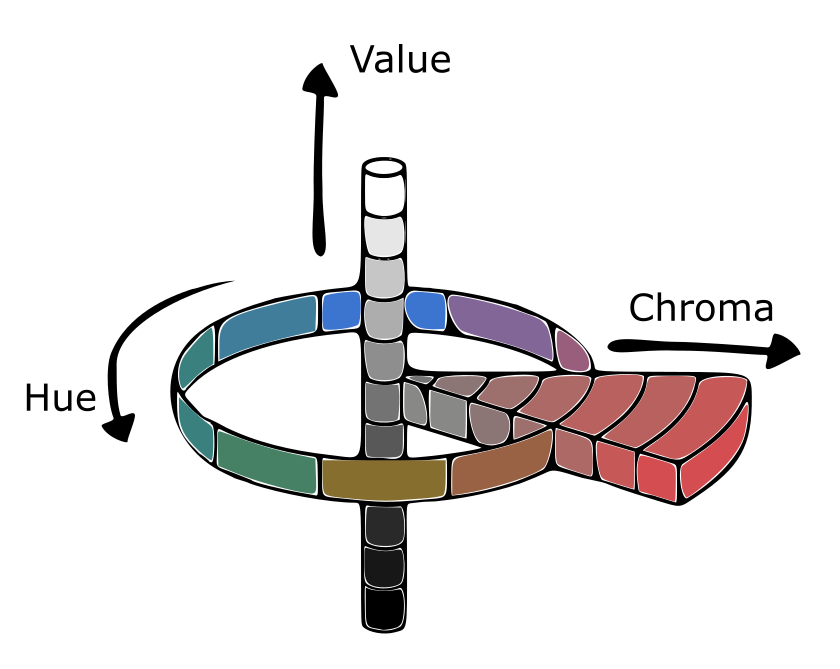
\includegraphics[width=0.4\linewidth]{image/general/munsell.png}  &
 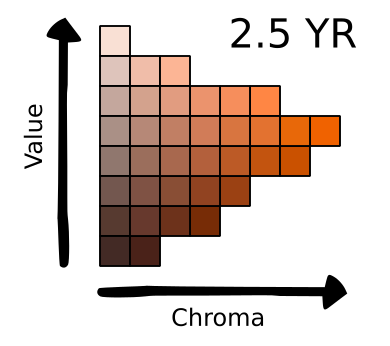
\includegraphics[width=0.4\linewidth]{image/general/25YR.png}\\
 (a) Munsell Color System &
(b) Hue at 2.5YR with various Chroma and Value\\
\end{tabular}
\caption{Munsell Color System} \label{fig:munsell}
\end{figure}


\section{Related work (STOA)}
\label{section:litreview}

